\todo[inline]{results}

\subsection{Nuclear Spin Mapping Fidelity}
\todo[inline]{Discuss all results related to nuclear spin mapping}

	As discussed earlier\todo{cite section}, nuclear spin mapping was used to improve the readout fidelity of our experiment. However, the improvement in fidelity was conditional upon the initial state of the electron at the time of the mapping. To perform correct mapping, a spin-down electron is required. Figure \ref{fig::wait_time} shows the total experimental error as a function of steering time. As steering time increases, we are more confident that the state of the electron was spin-down at the time of mapping, which is reflected in our decrease in error. The average time spent in the initialisation period is plotted on the right-axis. This would exceed the steering time in the average case, as a blip in current would require postponement of the donor plunge.
	\begin{figure}[htbp!]
		\centering
		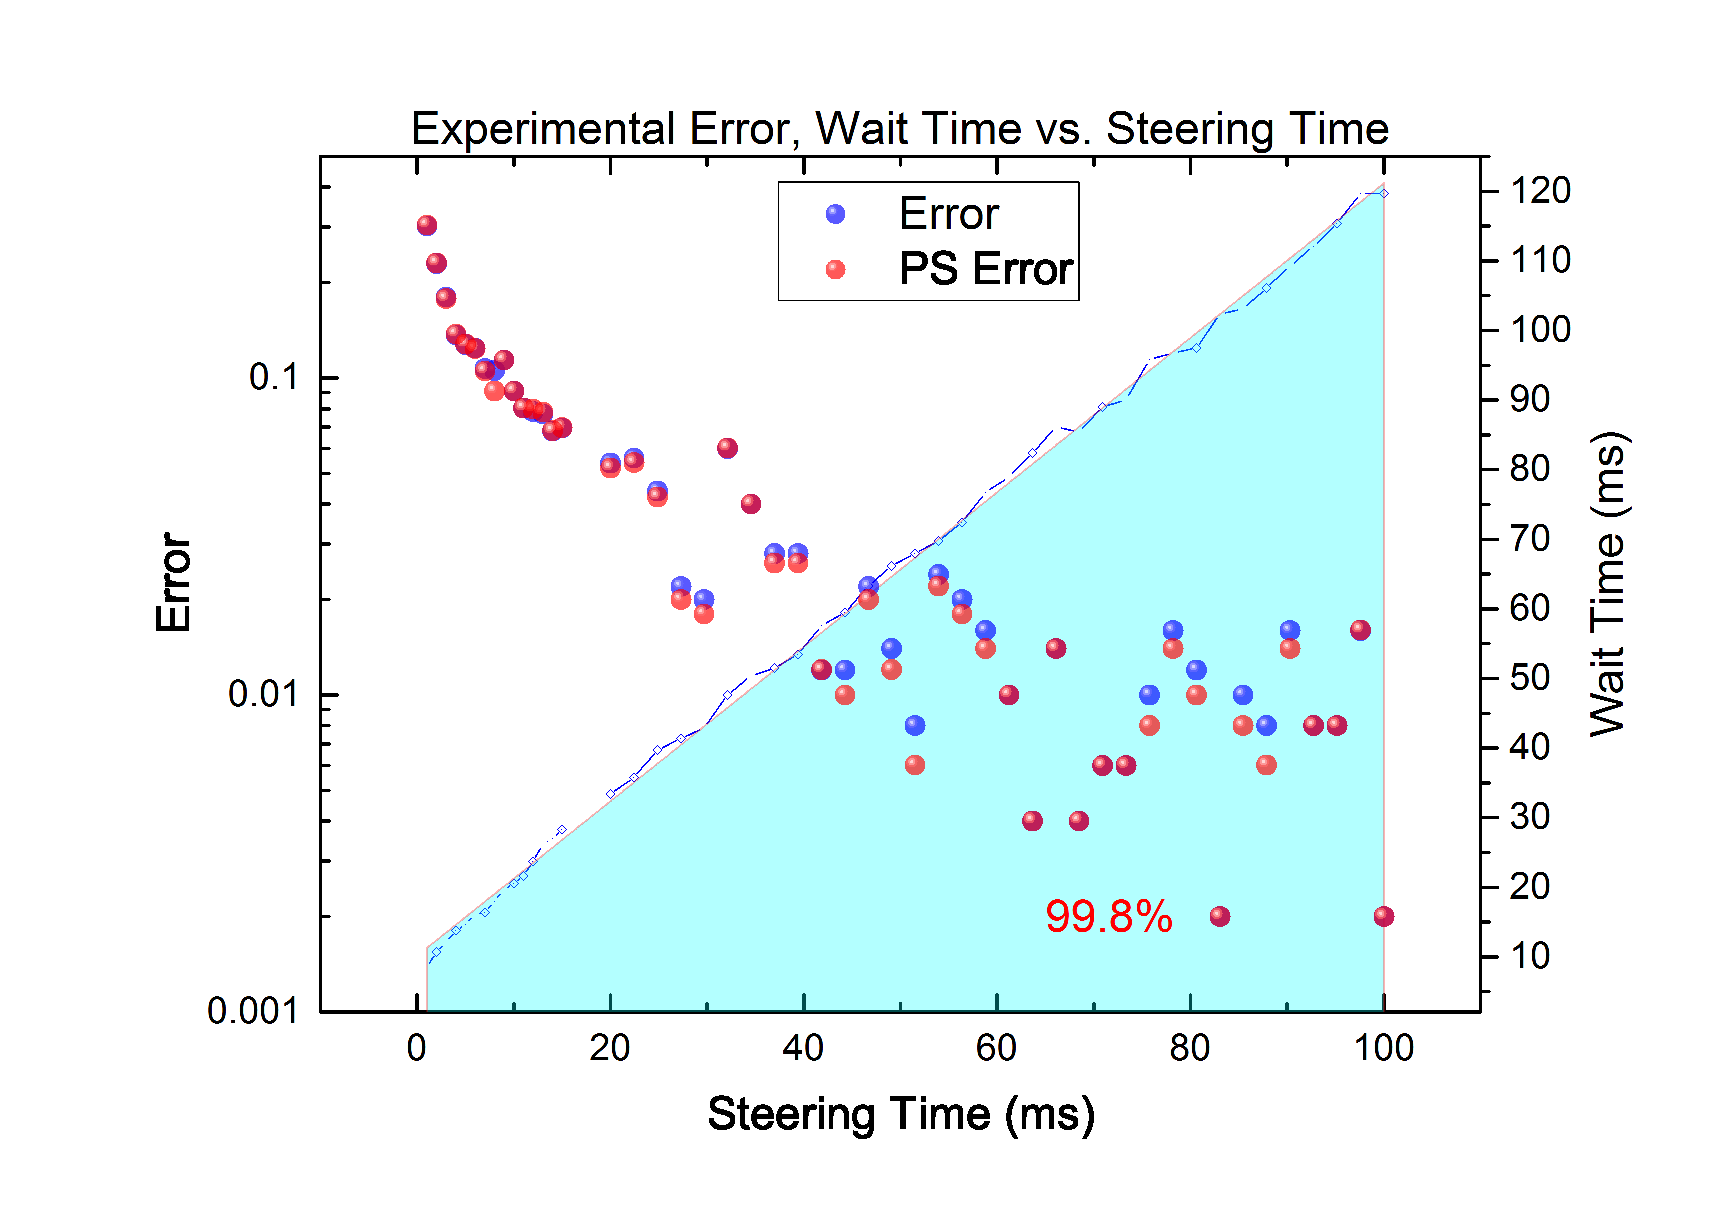
\includegraphics[width=0.8\textwidth]{WaitTimeFigLog}
		\caption{For a field of $B = 1$ T, the experimental error is plotted against steering time. On  the right axis is the average time spent at the initialisation level during the experiment.}
		\label{fig::wait_time}
	\end{figure}
	
	There are 2 separate data sets plotted, one for $B = 1.4$ T and the other for $B = 1$ T. These two datasets show the relationship between the required steering time for a good initialisation and the apparent tunnelling time of the donor electron. The required steering time to achieve 99\% fidelity is much longer for $B = 1$ T, however it was observed that the average tunnel time had not increased by such a margin from $B = 1.4$ T. This could be explained if we accept that the probability of a spin-down electron tunnelling off during the initialisation phase is high (also known as a dark-count), which is equivalent to a read-error. Whilst this is a possible explanation, it's not clear if this is accurate, and more examination of the data is required.

\subsection{Nuclear and Electron Rabi Oscillations}
	\todo[inline]{Discuss results pertaining to a high fidelity readout from a nuclear/electron rabi}

\subsection{Initialisation Level Tuning}
	The initialisation level of the pulse sequence was tuned to find the best position for a high fidelity experiment. It was discovered, however, that with initialisation there was a broad (approximately 400 mV) flat-band in which high fidelity results were obtained. This indicates another benefit in performing electron initialisation, which is insensitivity to tuning. This is a very useful property for a quantum computer, as reproducibility of measurements is crucial in determining the result of a computation.
	
	\todo[inline]{include graphic}
	Another novel application of this measurement is that we can infer the donor temperature from the width of the flat-band. The flat-band itself is a measure of the tail reading from the Zeeman splitting of the electron donor, assuming finite temperature.

